\documentclass[12pt,aspectratio=169]{beamer}
\usepackage[T1]{fontenc}
\usepackage{lmodern}
\usepackage{amsmath,amssymb,array,booktabs,tabularx,tikz}
% Add language support appropriate to the source, if needed.
% Keep this preamble inline in every delivered deck.
\definecolor{GEInk}{HTML}{132A3E}
\definecolor{GETeal}{HTML}{17675E}
\definecolor{GEFooter}{HTML}{EAF2F1}
\setbeamercolor{background canvas}{bg=white}
\setbeamercolor{normal text}{fg=GEInk,bg=white}
\setbeamercolor{structure}{fg=GETeal}
\setbeamercolor{frametitle}{fg=GEInk}
\setbeamercolor{GE footer}{fg=GETeal,bg=GEFooter}
\setbeamerfont{normal text}{family=\sffamily,size=\normalsize}
\setbeamerfont{title}{size=\huge,series=\bfseries}
\setbeamerfont{subtitle}{size=\normalsize,series=\bfseries}
\setbeamerfont{frametitle}{size=\Large,series=\bfseries}
\setbeamerfont{framesubtitle}{size=\normalsize,series=\mdseries}
\setbeamerfont{GE footer}{size=\footnotesize}
\setbeamersize{text margin left=9mm,text margin right=9mm}
\setbeamertemplate{navigation symbols}{}
\setbeamertemplate{headline}{}
\setbeamercovered{invisible}
\setbeamertemplate{frametitle}{%
  \vskip.5em
  {\usebeamerfont{frametitle}\strut\insertframetitle\strut\par}%
  \ifx\insertframesubtitle\empty\else
    {\usebeamerfont{framesubtitle}\strut\insertframesubtitle\strut\par}%
  \fi
  \vskip.25em
}
\setbeamertemplate{footline}{%
  \begin{beamercolorbox}[wd=\paperwidth,ht=3ex,dp=1.3ex,
    leftskip=9mm,rightskip=9mm]{GE footer}%
    \usebeamerfont{GE footer}\insertsectionhead\hfill
    \insertframenumber/\inserttotalframenumber
  \end{beamercolorbox}%
}
\setlength{\parindent}{0pt}
\setlength{\parskip}{.35em}
\setlength{\tabcolsep}{4pt}
\renewcommand{\arraystretch}{1.22}
\AtBeginEnvironment{frame}{\raggedright}
\addtobeamertemplate{frametitle}{}{%
  \setlength{\abovedisplayskip}{6pt plus 2pt minus 2pt}%
  \setlength{\belowdisplayskip}{6pt plus 2pt minus 2pt}%
  \setlength{\abovedisplayshortskip}{6pt plus 2pt minus 2pt}%
  \setlength{\belowdisplayshortskip}{6pt plus 2pt minus 2pt}%
}


\usetikzlibrary{arrows.meta,positioning,calc}
\usepackage{cancel}
% Source map: book2026-2027/fundamentals/permutations1.tex, lines 51--80:
% Introduction: Counting Choices, stopping BEFORE Worked Examples (line 82).
% Frames 2--4: multiplication paragraph; 5--8: factorial bullet;
% 9--12: ordered positions bullet; 13--16: unordered groups bullet;
% 17--20: indistinguishable copies bullet; 21--26: synthesis/oral checks.
% All small illustrations are authorized explanatory additions, not source exercises.
% No classroom activity, official criteria, lesson metadata, or highlight registry
% is supplied for this introduction. No invented legend/criteria/semantic colors.
% The starter's typography, structural colors, margins and logical footer are kept.
% All content is ink on white; no semantic highlights to disable.
\tikzset{card/.style={draw=GEInk,rounded corners=1mm,minimum width=10mm,
 minimum height=10mm,inner sep=2pt,font=\large\bfseries},
 box/.style={draw=GEInk,rounded corners=1mm,inner sep=5pt,align=center},
 link/.style={-{Stealth[length=2mm]},draw=GEInk},
 every picture/.style={draw=GEInk,text=GEInk,line width=.7pt}}
\newcommand{\question}[1]{{\bfseries #1}\par}
\newcommand{\captionline}[1]{\par{\small #1\par}}
\newcommand{\Row}[1]{\begin{tikzpicture}[baseline=-.5ex]
 \foreach \v [count=\j from 0] in {#1}{\node[card] at (1.15*\j,0){$\v$};}
 \end{tikzpicture}}
\newcommand{\Shirt}[3]{\begin{scope}[shift={(#1,#2)}]
 \draw (-.28,.4)--(-.58,.17)--(-.4,-.07)--(-.27,.04)--(-.27,-.48)
 --(.27,-.48)--(.27,.04)--(.4,-.07)--(.58,.17)--(.28,.4);
 \draw (-.28,.4) .. controls (-.12,.16) and (.12,.16) .. (.28,.4);
 \node[font=\small] at (0,-.16){#3};\end{scope}}
\newcommand{\DrawHat}[3]{\begin{scope}[shift={(#1,#2)}]
 \draw (-.58,-.2)--(.58,-.2)--(.58,-.08)--(.3,-.08)--(.23,.4)
 --(-.23,.4)--(-.3,-.08)--(-.58,-.08)--cycle;
 \node[font=\small] at (0,.1){#3};\end{scope}}
\newcommand{\Outfit}[2]{\begin{tikzpicture}[baseline=-.5ex]
 \path[use as bounding box] (-.65,-.55) rectangle (1.85,.55);
 \Shirt{0}{0}{S#1}\DrawHat{1.2}{0}{H#2}\end{tikzpicture}}
\newcommand{\SixRows}[1]{\begin{tikzpicture}
 \path[use as bounding box] (-.7,-1.9) rectangle (11.3,.7);
 \foreach \row [count=\j from 0] in {#1}{
  \pgfmathtruncatemacro{\col}{mod(\j,3)}
  \pgfmathtruncatemacro{\rr}{floor(\j/3)}
  \node[box,minimum width=3.1cm,minimum height=1cm,font=\Large]
   at (4*\col,-1.55*\rr){$\row$};}
 \end{tikzpicture}}
\title{Introduction: Counting Choices}
\author{}\date{}
\begin{document}
\section{Counting choices}
\begin{frame}
\vfill
{\huge\bfseries Introduction:\\Counting Choices\par}
\bigskip
How can we count every possibility\par without missing any or counting twice?
\bigskip
\par{\centering \Row{A,B,C}\quad\Row{B,A,C}\par}
\captionline{The same cards can make different rows.}
\vfill
\end{frame}

\section{Multiply choices}
% Teaching note: Collect predictions; do not confirm six until the tree is built.
\begin{frame}[t]{One shirt and one hat}

\question{Predict: how many different outfits can we make?}
Choose exactly one shirt and exactly one hat.
\par{\centering 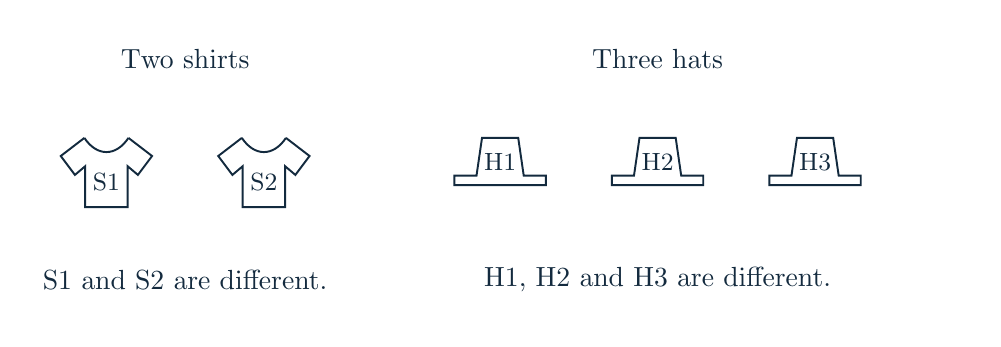
\begin{tikzpicture}
\path[use as bounding box] (-1,-1.1) rectangle (11,2.6);
\node at (1,2.2){Two shirts};\node at (7,2.2){Three hats};
\Shirt{0}{.8}{S1}\Shirt{2}{.8}{S2}
\DrawHat{5}{.8}{H1}\DrawHat{7}{.8}{H2}\DrawHat{9}{.8}{H3}
\node at (1,-.6){S1 and S2 are different.};
\node at (7,-.6){H1, H2 and H3 are different.};
\end{tikzpicture}\par}
\visible<2->{Every shirt can go with every hat.}
\captionline{Labels identify the choices, even without color.}

\end{frame}

\section{Multiply choices}
% Teaching note: Trace one complete path. A partial path is not an outfit.
\begin{frame}[t]{A tree shows every outfit}

\question{After either shirt, how many hat choices remain?}
\par{\centering 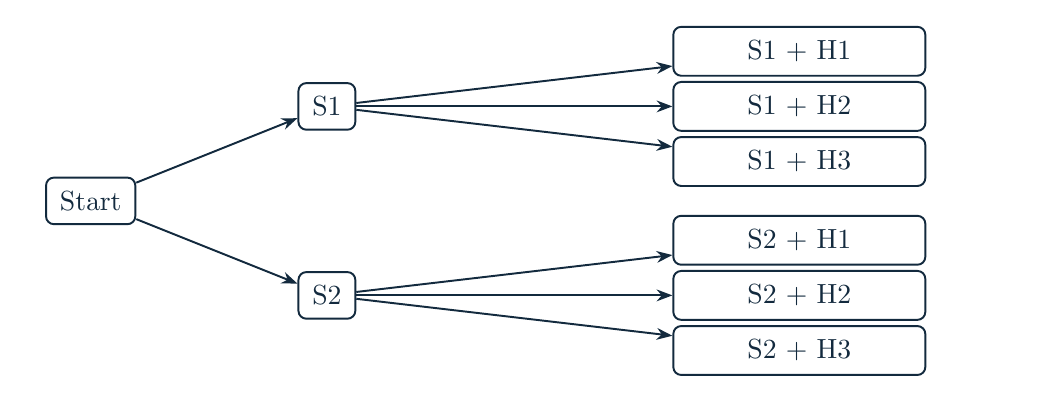
\begin{tikzpicture}
\path[use as bounding box] (-.8,-.6) rectangle (11.7,3.7);
\node[box] (start) at (0,1.5){Start};
\visible<2->{\node[box] (s1) at (3,2.7){S1};\node[box] (s2) at (3,.3){S2};
 \draw[link] (start)--(s1);\draw[link] (start)--(s2);}
\foreach \s/\base/\ov in {1/2.7/3,2/.3/4}{
 \foreach \h/\dy in {1/.7,2/0,3/-.7}{
 \visible<\ov->{\node[box,minimum width=3.2cm] (o\s\h) at (9,\base+\dy){S\s\ + H\h};
 \draw[link] (s\s)--(o\s\h);}}}
\end{tikzpicture}\par}
\visible<4->{\captionline{Each complete path gives one outfit: three on each shirt branch.}}

\end{frame}

\section{Multiply choices}
% Teaching note: Here two choices at step one and three at step two; they need not equal each other.
\begin{frame}[t]{A grid turns counting into multiplication}

\question{How many outfits are in each row?}
\par{\centering 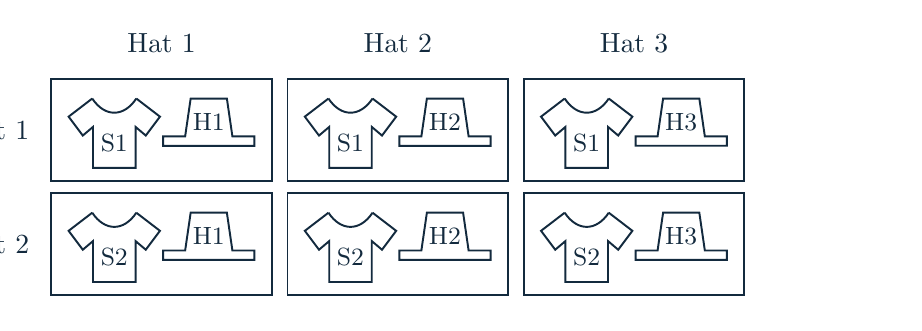
\begin{tikzpicture}
\path[use as bounding box] (-1.7,-2.6) rectangle (9.3,.9);
\foreach \h in {1,2,3}{\node at (3*\h-3,.7){Hat \h};}
\foreach \s/\y/\ov in {1/-.4/2,2/-1.85/3}{
 \node[anchor=east] at (-1.55,\y){Shirt \s};
 \foreach \h in {1,2,3}{\draw (3*\h-4.4,\y-.65) rectangle (3*\h-1.6,\y+.65);
 \visible<\ov->{\node at (3*\h-3,\y){\Outfit{\s}{\h}};}}}
\end{tikzpicture}\par}
\visible<3->{$3+3=2\times3=6$ outfits. Two rows, three in each row.}
\visible<4->{\par\textbf{Multiplication principle:} every earlier choice must leave the
same number of choices at the next step. The numbers can differ between steps.}

\end{frame}

\section{Arrange all cards}
% Teaching note: The crossed cards are already in the row, not discarded. ABC is only one possible path.
\begin{frame}[t]{Fill three positions, using each card once}

\question{Predict: how many different rows can A, B and C make?}
\par{\centering 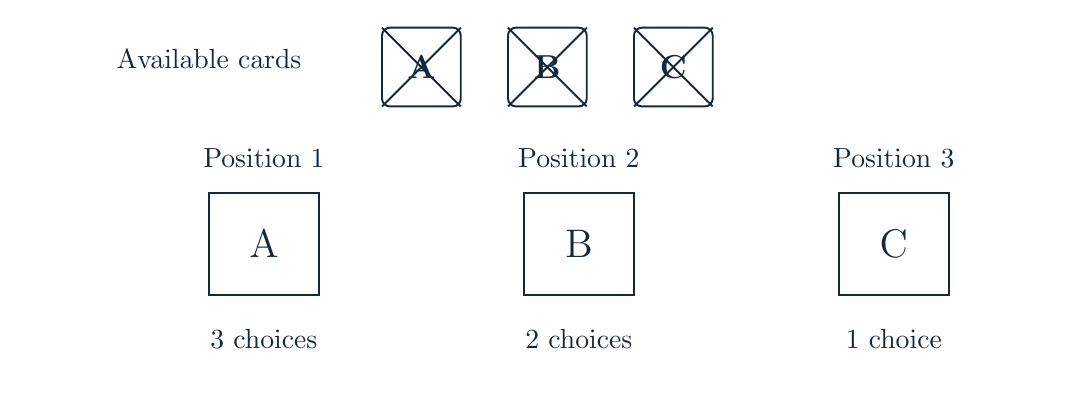
\begin{tikzpicture}
\path[use as bounding box] (-1,-.8) rectangle (12,3.5);
\node[anchor=west] at (0,3.1){Available cards};
\foreach \v [count=\j from 0] in {A,B,C}{\node[card] at (4+1.6*\j,3){\v};}
\visible<2->{\draw (3.5,2.5)--(4.5,3.5);\draw (3.5,3.5)--(4.5,2.5);}
\visible<3->{\draw (5.1,2.5)--(6.1,3.5);\draw (5.1,3.5)--(6.1,2.5);}
\visible<4->{\draw (6.7,2.5)--(7.7,3.5);\draw (6.7,3.5)--(7.7,2.5);}
\foreach \x/\p/\v/\ov/\count in {2/1/A/2/3,6/2/B/3/2,10/3/C/4/1}{
 \node at (\x,1.85){Position \p};\draw (\x-.7,.1) rectangle (\x+.7,1.4);
 \visible<\ov->{\node[font=\Large] at (\x,.75){\v};\node at (\x,-.45){\count\ \ifnum\count=1 choice\else choices\fi};}}
\end{tikzpicture}\par}
\visible<4->{$3\times2\times1=6$. Used cards cannot be chosen again.}
\visible<4->{\captionline{One path is shown. Any first card leaves two, then one.}}

\end{frame}

\section{Arrange all cards}
% Teaching note: Ask students to check completeness by grouping rows by their first letter.
\begin{frame}[t]{Here are all six arrangements}

\question{Does swapping A and B make a different row?}
\par{\centering 
\visible<2->{\SixRows{ABC,ACB,BAC,BCA,CAB,CBA}}
\par}
\visible<3->{Yes: ABC and BAC have different cards in their positions.
\[3\times2\times1=6=3!\]}
\visible<3->{The symbol $!$ means \textbf{factorial}: multiply down to 1.
Read $3!$ as ``three factorial.''}
\visible<3->{\captionline{Two rows start with each possible first card.}}

\end{frame}

\section{Arrange all cards}
% Teaching note: This is the first use of n. Factorial is not multiplication by the punctuation mark.
\begin{frame}[t]{A short name for a decreasing product}

\question{Predict: how would you count rows of four different cards?}
\par{\centering \Row{A,B,C,D}\par}
\visible<2->{\[4\times3\times2\times1=24=4!\]}
\visible<3->{Let $n$ mean the \textbf{total number of different objects}.
For at least one object:
\[\boxed{n!=n\times(n-1)\times\cdots\times2\times1}\]
$n-1$ means one fewer than $n$; $\cdots$ means keep decreasing by 1.
There is one factor for each position.}
\visible<2->{\captionline{Every position uses one object, leaving one fewer choice.}}

\end{frame}

\section{Arrange all cards}
% Teaching note: Distinguish zero objects from zero arrangements. We count the one empty result.
\begin{frame}[t]{One card --- and no cards}

\question{Predict: how many rows can you make with one card? With none?}
\par{\centering 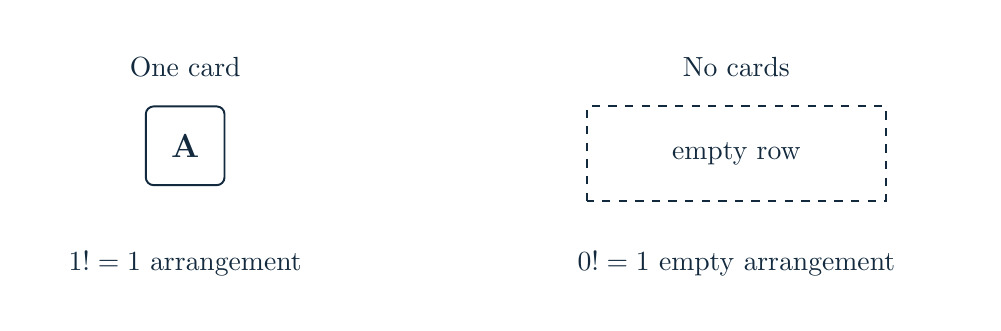
\begin{tikzpicture}
\path[use as bounding box] (-2,-1.3) rectangle (10,2.2);
\node at (0,1.7){One card};\node at (7,1.7){No cards};
\node[card] at (0,.7){A};
\draw[dashed] (5.1,0) rectangle (8.9,1.2);
\node at (7,.6){empty row};
\visible<2->{\node at (0,-.8){$1!=1$ arrangement};}
\visible<3->{\node at (7,-.8){$0!=1$ empty arrangement};}
\end{tikzpicture}\par}
\visible<3->{There is exactly one way to leave all positions empty.
So we define zero factorial to be 1.}
\captionline{The dashed outline shows an empty row, not an extra object.}

\end{frame}

\section{Fill some positions}
% Teaching note: Names A--D identify four different students. The jobs are ordered positions, not a team.
\begin{frame}[t]{Four students, two different jobs}

\question{Predict: how many ways can we assign the jobs?}
The students are A, B, C and D. Each student can do at most one job.
\par{\centering \Row{A,B,C,D}\par\medskip
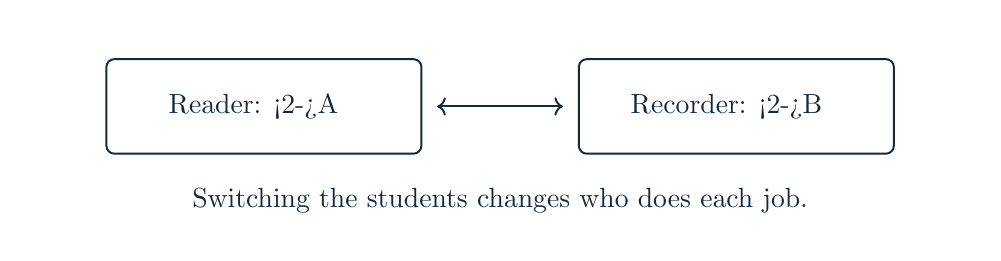
\begin{tikzpicture}
\path[use as bounding box] (-2,-.9) rectangle (10,1.7);
\node[box,minimum width=4cm,minimum height=1.2cm] at (1,.7){Reader: \alt<2->{A}{\phantom{A}}};
\node[box,minimum width=4cm,minimum height=1.2cm] at (7,.7){Recorder: \alt<2->{B}{\phantom{B}}};
\draw[<->] (3.2,.7)--(4.8,.7);
\node at (4,-.5){Switching the students changes who does each job.};
\end{tikzpicture}\par}
\visible<2->{A as reader and B as recorder differs from B as reader and A as recorder.}

\end{frame}

\section{Fill some positions}
% Teaching note: Read all twelve leaves; check that each reader branch excludes the same student below it.
\begin{frame}[t]{A complete tree: four branches, three each}

\question{After choosing the reader, who can be the recorder?}
\par{\centering 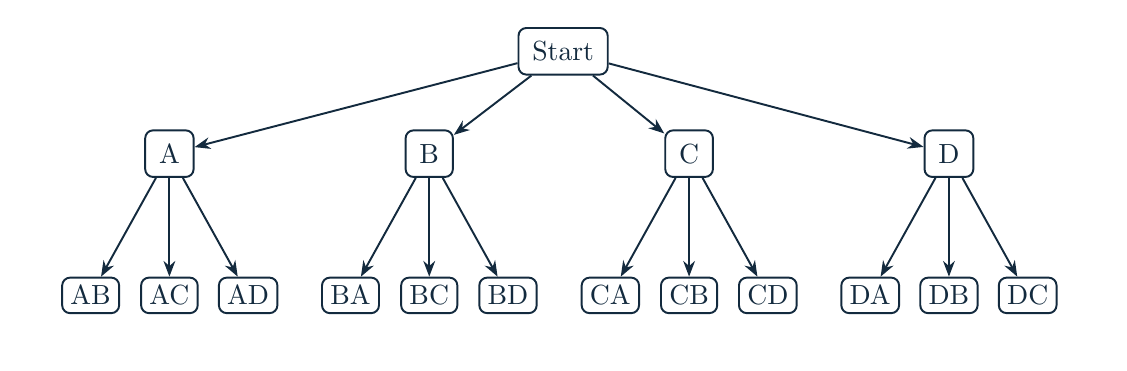
\begin{tikzpicture}
\path[use as bounding box] (-.8,-.4) rectangle (12.8,3.6);
\node[box] (start) at (6,3.3){Start};
\foreach \a/\x/\others in {A/1/{B,C,D},B/4.3/{A,C,D},C/7.6/{A,B,D},D/10.9/{A,B,C}}{
 \visible<2->{\node[box] (r\a) at (\x,2){\a};\draw[link] (start)--(r\a);}
 \foreach \b [count=\j from 0] in \others {
 \visible<3->{\node[box,inner sep=3pt] (p\a\b) at (\x-1+\j,.2){\a\b};
 \draw[link] (r\a)--(p\a\b);}}}
\end{tikzpicture}\par}
\visible<3->{$4\times3=12$ job assignments. No AA, BB, CC or DD is allowed.}
\visible<3->{\captionline{First letter = reader; second letter = recorder. Every reader leaves three choices.}}

\end{frame}

\section{Fill some positions}
% Teaching note: Cancellation divides equal nonzero factors. We are not dividing away the two job orders.
\begin{frame}[t]{Why divide a factorial?}

\question{We stop after two jobs. Which factors should we keep?}
\par{\centering 
\begin{tikzpicture}
\path[use as bounding box] (-1,-.45) rectangle (12,.8);
\foreach \x/\v/\lab in {0/4/Reader,3/3/Recorder,6/2/Unused,9/1/Unused}{
 \node[box,inner sep=3pt,minimum width=1.4cm,font=\Large] at (\x,.4){\v};
 \node[font=\small] at (\x,-.3){\lab};}
\end{tikzpicture}\par}
\visible<2->{All four positions would give $4!=4\times3\times2\times1$.}
\begin{overlayarea}{\linewidth}{2.7cm}
\visible<2->{\[\frac{4!}{2!}=
\frac{4\times3\times\underbrace{(\alt<3->{\cancel{2}}{2}\times\alt<3->{\cancel{1}}{1})}_{2!}}
{\underbrace{\alt<3->{\cancel{2}}{2}\times\alt<3->{\cancel{1}}{1}}_{2!}}
\visible<3->{=4\times3=12}\]}
\end{overlayarea}
\visible<2->{\captionline{Divide away the unused tail. Keep only the two job choices.}}

\end{frame}

\section{Fill some positions}
% Teaching note: For r=0 there is one empty assignment (empty product); r=n gives n!/0!=n!.
\begin{frame}[t]{The rule for some ordered positions}

\question{What if there are more objects and more jobs?}
\visible<2->{Let $n$ be the number of distinct available objects.
Let $r$ be the number of ordered positions to fill.
Then $n-r$ counts the objects left unused.}
\visible<3->{\[
\underbrace{n\times(n-1)\times\cdots\times(n-r+1)}_{r\text{ decreasing choice counts}}
=\boxed{\frac{n!}{(n-r)!}}
\]}
\visible<3->{$n-r+1$ is the number left for the last position:
we have already used $r-1$ objects.}
\visible<4->{For our jobs: $n=4$, $r=2$, $n-r=2$.
The retained factors are $4$ and $3$.}
\visible<4->{\captionline{Use each object at most once. Choose a whole number $r$ from 0 to $n$; $r=0$ gives one empty assignment.}}

\end{frame}

\section{Choose a group}
% Teaching note: Order of listing does not create a new membership. No student is repeated within a team.
\begin{frame}[t]{Same students, but now choose a team}

\question{Predict: are there still 12 different two-person teams?}
Choose two of A, B, C and D. There are \textbf{no jobs}.
\par{\centering 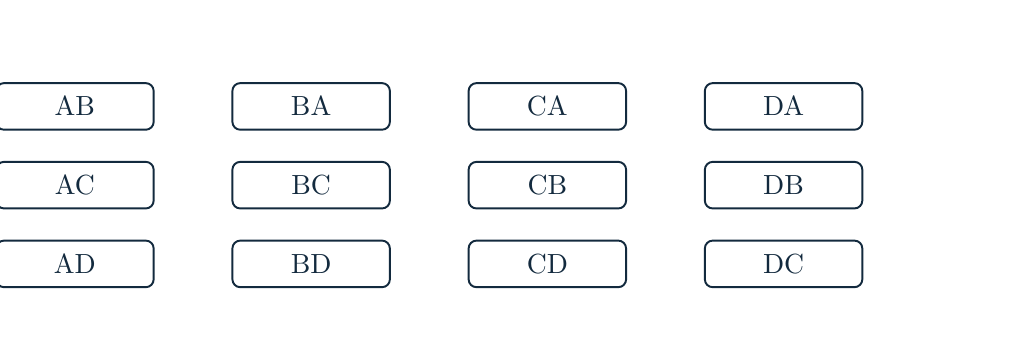
\begin{tikzpicture}
\path[use as bounding box] (-.6,-2.8) rectangle (11.8,1);
\foreach \a/\x/\others in {A/0/{B,C,D},B/3/{A,C,D},C/6/{A,B,D},D/9/{A,B,C}}{
 \foreach \b [count=\j from 0] in \others{
 \visible<2->{\node[box,minimum width=2cm] at (\x,-\j){\a\b};}}}
\end{tikzpicture}\par}
\visible<3->{AB and BA list the \textbf{same members}. They are one team.}
\captionline{These are the 12 ordered lists from the job tree. Look for repeated teams.}

\end{frame}

\section{Choose a group}
% Teaching note: Point to all six boxes. Division works because EVERY team has exactly two lists.
\begin{frame}[t]{Pair the lists that name the same team}

\question{How many lists name each two-person team?}
\par{\centering 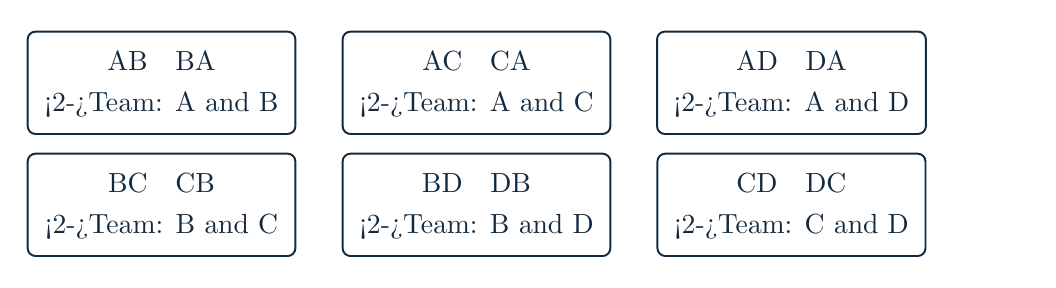
\begin{tikzpicture}
\path[use as bounding box] (-.7,-2.25) rectangle (12,.7);
\foreach \a/\b/\x/\y in {A/B/1/0,A/C/5/0,A/D/9/0,B/C/1/-1.55,B/D/5/-1.55,C/D/9/-1.55}{
 \node[box,inner sep=2pt,minimum width=3.4cm,minimum height=1.3cm] at (\x,\y){
 \begin{tabular}{c}\a\b\quad\b\a\\\visible<2->{Team: \a\ and \b}\end{tabular}};}
\end{tikzpicture}\par}
\visible<3->{Each team appears $2!=2$ times.
\[12\div2!=12\div2=6\text{ distinct teams}\]}
\captionline{Each box is one team; both lists inside it have the same membership.}

\end{frame}

\section{Choose a group}
% Teaching note: This is one team, not six teams. The factorial counts its possible lists.
\begin{frame}[t]{Why does a bigger group need a bigger divisor?}

\question{How many ordered lists name the single team A, B, C?}
\par{\centering \visible<2->{\SixRows{ABC,ACB,BAC,BCA,CAB,CBA}}\par}
\visible<3->{All six lists name \textbf{one team}.
Three members have $3!=3\times2\times1=6$ orders.}
\visible<4->{A team with $r$ members has $r!$ orders.
So the ordered count includes \textbf{every team exactly $r!$ times}.}
\captionline{Changing the list changes positions, but it does not change membership.}

\end{frame}

\section{Choose a group}
% Teaching note: In 4 choose 2 the two 2! factors have different reasons, even though their values match.
\begin{frame}[t]{Count each team just once}

\question{Which repeated counting should we divide away?}
\visible<2->{First count ordered choices; then divide by the orders of each team.
\par Teams = ordered choices $\div$ orders per team.}
\visible<3->{\[\boxed{\binom nr=\frac{n!}{r!(n-r)!}}\]
Read $\binom nr$ as ``$n$ choose $r$.'' It counts groups without roles.}
\visible<4->{\[\binom42=\frac{4!}{2!\,2!}=\frac{12}{2}=6\text{ teams}\]}
\visible<4->{\captionline{One denominator removes unused factors; the other removes repeated team orders.}}

\end{frame}

\section{Identical copies}
% Teaching note: Do not reveal three visible rows yet. Ask which labelled rows will become indistinguishable.
\begin{frame}[t]{Two A cards and one B card}

\question{Predict: how many different visible rows can A, A, B make?}
\par{\centering \Row{A,A,B}\par}
\visible<2->{Give the A copies temporary labels $A_1$ and $A_2$: copy 1 and copy 2.}
\par{\centering \visible<3->{\SixRows{A_1A_2B,A_2A_1B,A_1BA_2,A_2BA_1,BA_1A_2,BA_2A_1}}\par}
\visible<3->{Three different \emph{labelled} cards give $3!=6$ rows.}
\captionline{Temporary labels let us count first; they are not on the real cards.}

\end{frame}

\section{Identical copies}
% Teaching note: All three supplied cards appear once in each visible row. Identical does not mean reusable.
\begin{frame}[t]{Erase labels and group the matching rows}

\question{Which rows become the same when 1 and 2 disappear?}
\par{\centering 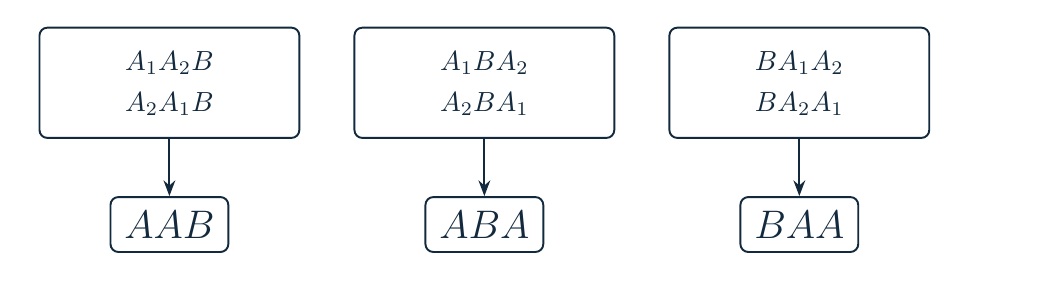
\begin{tikzpicture}
\path[use as bounding box] (-.8,-1.85) rectangle (12,1.1);
\foreach \x/\one/\two/\plain in {1/{A_1A_2B}/{A_2A_1B}/{AAB},5/{A_1BA_2}/{A_2BA_1}/{ABA},9/{BA_1A_2}/{BA_2A_1}/{BAA}}{
 \node[box,minimum width=3.3cm,minimum height=1.4cm] (g\x) at (\x,.4){
 \begin{tabular}{c}$\one$\\$\two$\end{tabular}};
 \visible<2->{\node[box,font=\Large] (v\x) at (\x,-1.4){$\plain$};
 \draw[link] (g\x)--(v\x);}}
\end{tikzpicture}\par}
\visible<3->{Each visible row was counted $2!=2$ times.
\[\frac{3!}{2!}=\frac{6}{2}=3\text{ visible arrangements}\]}
\visible<3->{\captionline{Swapping identical A copies makes no visible change.}}

\end{frame}

\section{Identical copies}
% Teaching note: Each visible arrangement has four labelled versions, even if identical copies are not adjacent.
\begin{frame}[t]{Two repeated types: A, A, B, B}

\question{How many labelled rows become this one visible row: AABB?}
\par{\centering 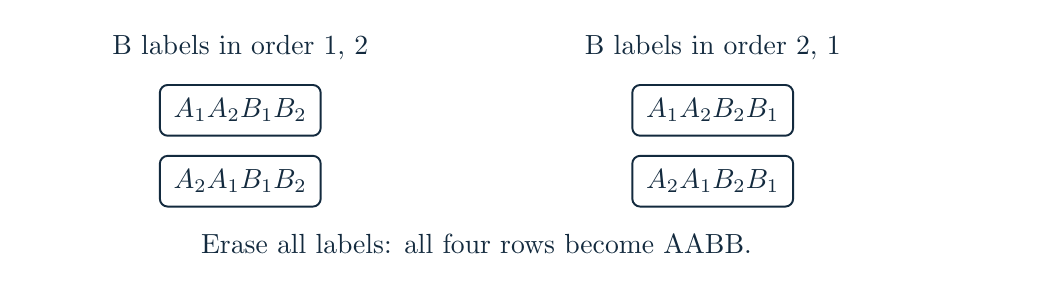
\begin{tikzpicture}
\path[use as bounding box] (-.7,-2) rectangle (12,.95);
\node at (2,.7){B labels in order 1, 2};\node at (8,.7){B labels in order 2, 1};
\visible<2->{
\node[box] at (2,-.1){$A_1A_2B_1B_2$};\node[box] at (8,-.1){$A_1A_2B_2B_1$};
\node[box] at (2,-1){$A_2A_1B_1B_2$};\node[box] at (8,-1){$A_2A_1B_2B_1$};
\node at (5,-1.8){Erase all labels: all four rows become AABB.};}
\end{tikzpicture}\par}
\visible<3->{Every row: $2!$ A-label orders $\times$ $2!$ B-label orders $=4$.
\[\frac{4!}{2!\,2!}=\frac{24}{4}=6\]}
\visible<4->{\captionline{Check the six: AABB, ABAB, ABBA, BAAB, BABA, BBAA.}}

\end{frame}

\section{Identical copies}
% Teaching note: The source uses m_i: i is any type number from 1 to k. Label swaps are independent across types.
\begin{frame}[t]{The rule for indistinguishable copies}

\question{What must we divide away for every repeated type?}
\visible<2->{Use all $n$ supplied objects. Let $k$ be the number of types.
Let $m_1,m_2,\ldots,m_k$ count the copies of types $1,2,\ldots,k$.
Each count is a positive whole number, and
\[m_1+m_2+\cdots+m_k=n.\]}
\visible<3->{\[\boxed{\text{visible rows}=\frac{n!}{m_1!m_2!\cdots m_k!}}\]
There are $n!$ labelled rows. Each visible row has
$m_1!\times m_2!\times\cdots\times m_k!$ label orders.}
\visible<4->{\textbf{Identical copies are not reuse:} every supplied card is placed exactly once.}
\visible<2->{\captionline{A subscript identifies a type; the dots mean continue through all $k$ types.}}

\end{frame}

\section{Synthesis}
% Teaching note: For a group, exchanging list positions leaves membership unchanged. The repeated-copy formula here arranges ALL copies.
\begin{frame}[t]{Choose a route before choosing a formula}

\question{Are we arranging objects or choosing a group?}
\par{\centering 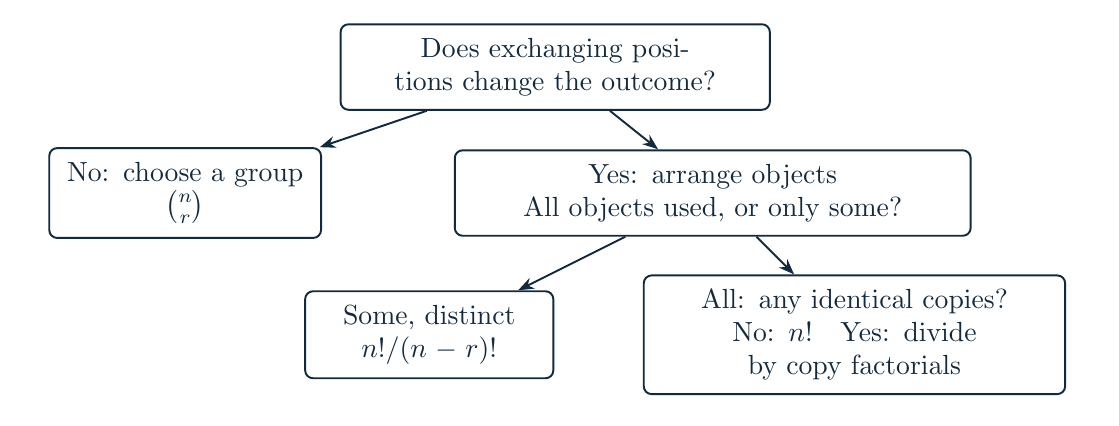
\begin{tikzpicture}
\path[use as bounding box] (-.5,-3.6) rectangle (13,1.1);
\node[box,text width=5.1cm] (q) at (6.2,.6){Does exchanging positions change the outcome?};
\visible<2->{
\node[box,text width=3.1cm] (g) at (1.5,-1){No: choose a group\\$\binom nr$};
\node[box,text width=6.2cm] (a) at (8.2,-1){Yes: arrange objects\\All objects used, or only some?};
\draw[link] (q)--(g);\draw[link] (q)--(a);}
\visible<3->{
\node[box,text width=2.8cm] (s) at (4.6,-2.8){Some, distinct\\$n!/(n-r)!$};
\node[box,text width=5cm] (all) at (10,-2.8){All: any identical copies?\\No: $n!$\quad Yes: divide by copy factorials};
\draw[link] (a)--(s);\draw[link] (a)--(all);}
\end{tikzpicture}\par}
\captionline{These routes assume the objects are used without replacement.}

\end{frame}

\section{Synthesis}
% Teaching note: Ask students to explain decreasing choices in words rather than recall formula names.
\begin{frame}[t]{Rules at a glance: steps and ordered positions}

\begin{columns}[T,onlytextwidth]
\begin{column}{.485\textwidth}
\textbf{Complete steps}
\par{\centering 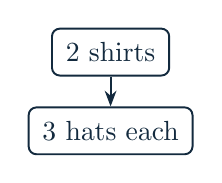
\begin{tikzpicture}
\node[box] (a) at (0,0){2 shirts};\node[box] (b) at (0,-1){3 hats each};
\draw[link] (a)--(b);\end{tikzpicture}\par}
Multiply step counts: $2\times3=6$.
Every earlier choice leaves the same next-step count.
\end{column}
\begin{column}{.485\textwidth}
\textbf{Distinct objects; order matters}
\par{\centering \Row{A,B,C}\par}
All $n$ objects: $n!$.
\medskip
\par{\centering 
\begin{tikzpicture}
\node[box] at (0,0){Reader};\node[box] at (2.3,0){Recorder};
\end{tikzpicture}\par}
Only $r$ positions: $\dfrac{n!}{(n-r)!}$.
\end{column}\end{columns}
\medskip\captionline{A row changes when different objects exchange positions.}

\end{frame}

\section{Synthesis}
% Teaching note: The reasons for division differ: listing a group versus labelling identical copies.
\begin{frame}[t]{Rules at a glance: groups and identical copies}

\begin{columns}[T,onlytextwidth]
\begin{column}{.485\textwidth}
\textbf{A group without roles}
\par{\centering 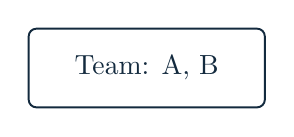
\begin{tikzpicture}
\node[box,minimum width=3cm,minimum height=1cm]{Team: A, B};
\end{tikzpicture}\par}
AB and BA are one team.
\[\binom nr=\frac{n!}{r!(n-r)!}\]
Divide by the $r!$ lists of each team.
\end{column}
\begin{column}{.485\textwidth}
\textbf{Arrange all identical copies}
\par{\centering \Row{A,A,B}\par}
Swapping the A copies changes nothing visible.
\[\frac{n!}{m_1!m_2!\cdots m_k!}\]
Divide by label orders within every type.
\end{column}\end{columns}
\medskip\captionline{In both rules, divide because each actual result was counted equally often.}

\end{frame}

\section{Oral checks}
% Teaching note: Wait for an explanation before advancing to the answer overlay.
\begin{frame}[t]{Oral check 1: outfits}

\question{Two shirts and two hats. Every hat fits with every shirt.}
How many outfits? Explain why multiplication works.
\par{\centering 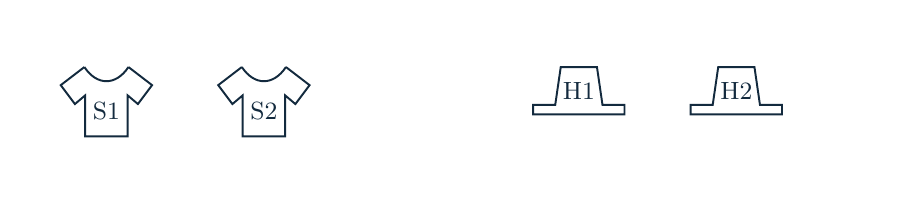
\begin{tikzpicture}
\path[use as bounding box] (-1,-.8) rectangle (10,1.3);
\Shirt{0}{.4}{S1}\Shirt{2}{.4}{S2}\DrawHat{6}{.4}{H1}\DrawHat{8}{.4}{H2}
\end{tikzpicture}\par}
\visible<2->{\textbf{Answer:} $2\times2=4$ outfits.
Either shirt leaves two hat choices.}
\visible<3->{\par{\centering 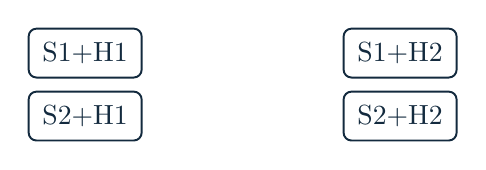
\begin{tikzpicture}
\foreach \x/\y/\v in {0/0/{S1+H1},4/0/{S1+H2},0/-.8/{S2+H1},4/-.8/{S2+H2}}{
\node[box] at (\x,\y){\v};}\end{tikzpicture}\par}}
\visible<3->{\captionline{Check the answer by listing all four complete outfits.}}

\end{frame}

\section{Oral checks}
% Teaching note: Seek the distinction between different jobs and a different listing of the same team.
\begin{frame}[t]{Oral check 2: jobs or a team?}

\question{Use A, B and C. No student can be used twice.}
How many reader--recorder assignments? How many two-person teams?
\par{\centering \Row{A,B,C}\par}
\visible<2->{\textbf{Jobs:} $3\times2=6$. Exchanging students changes the jobs.
\par{\centering 
\begin{tikzpicture}
\foreach \v [count=\j from 0] in {AB,AC,BA,BC,CA,CB}{\node[box] at (1.9*\j,0){\v};}
\end{tikzpicture}\par}}
\visible<3->{\textbf{Teams:} $6\div2!=3$. Each team has two lists.
\par{\centering 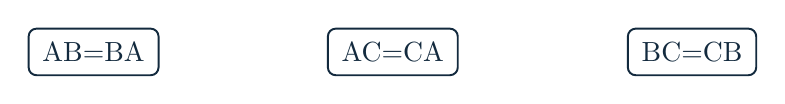
\begin{tikzpicture}
\foreach \v [count=\j from 0] in {AB=BA,AC=CA,BC=CB}{\node[box] at (3.8*\j,0){\v};}
\end{tikzpicture}\par}}
\visible<3->{\captionline{For the teams, the equals sign means ``same members.''}}

\end{frame}

\section{Oral checks}
% Teaching note: Finish by asking: what is one actual outcome, and how often did our first count include it?
\begin{frame}[t]{Oral check 3: identical cards}

\question{Use every card once: A, B, B. How many visible rows?}
Explain what must be divided away.
\par{\centering \Row{A,B,B}\par}
\visible<2->{\textbf{Answer:} $3!\div2!=6\div2=3$.
Temporary labels on the two B cards give two versions of each visible row.}
\par{\centering \visible<3->{
\begin{tikzpicture}
\path[use as bounding box] (-.7,-.6) rectangle (11.3,.6);
\foreach \v [count=\j from 0] in {ABB,BAB,BBA}{
\node[box,minimum width=3.1cm,minimum height=1cm,font=\Large] at (4*\j,0){$\v$};}
\end{tikzpicture}}\par}
\visible<3->{Every card is placed once. The B copies look the same; we do not reuse a card.}
\captionline{List the visible outcomes to verify the division.}

\end{frame}

\end{document}
